%%%%%%%%%%%%%%%%%%%%%%% file template.tex %%%%%%%%%%%%%%%%%%%%%%%%%
%
% This is a general template file for the LaTeX package SVJour3
% for Springer journals.          Springer Heidelberg 2010/09/16
%
% Copy it to a new file with a new name and use it as the basis
% for your article. Delete % signs as needed.
%
% This template includes a few options for different layouts and
% content for various journals. Please consult a previous issue of
% your journal as needed.
%
%%%%%%%%%%%%%%%%%%%%%%%%%%%%%%%%%%%%%%%%%%%%%%%%%%%%%%%%%%%%%%%%%%%
%
% First comes an example EPS file -- just ignore it and
% proceed on the \documentclass line
% your LaTeX will extract the file if required
\begin{filecontents*}{example.eps}
%!PS-Adobe-3.0 EPSF-3.0
%%BoundingBox: 19 19 221 221
%%CreationDate: Mon Sep 29 1997
%%Creator: programmed by hand (JK)
%%EndComments
gsave
newpath
  20 20 moveto
  20 220 lineto
  220 220 lineto
  220 20 lineto
closepath
2 setlinewidth
gsave
  .4 setgray fill
grestore
stroke
grestore
\end{filecontents*}
%
\RequirePackage{fix-cm}
%
%\documentclass{svjour3}                     % onecolumn (standard format)
%\documentclass[smallcondensed]{svjour3}     % onecolumn (ditto)
\documentclass[smallextended]{svjour3}       % onecolumn (second format)
%\documentclass[twocolumn]{svjour3}          % twocolumn
%
\smartqed  % flush right qed marks, e.g. at end of proof
%
\usepackage{graphicx}
%
% \usepackage{mathptmx}      % use Times fonts if available on your TeX system
%
% insert here the call for the packages your document requires
%\usepackage{latexsym}
% etc.
%
% please place your own definitions here and don't use \def but
% \newcommand{}{}
%
% Insert the name of "your journal" with
% \journalname{myjournal}
%
\begin{document}

\title{Blind prediction of cyclohexane-water distribution coefficients from the SAMPL5 challenge}
\thanks{NSF, green planet (their NSF), anything else?}

\subtitle{I don't think we need a subtitle...}

%\titlerunning{Short form of title}        % if too long for running head

\author{Caitlin C Bannan         \and
        Kalistyn H Burley \and
        David L Mobley
}

%\authorrunning{Short form of author list} % if too long for running head

\institute{C. C. Bannan, K. H. Burley, and D. L. Mobley \at University of California, Irvine \\
              Tel.: +123-45-678910\\
              Fax: +123-45-678910\\
              \email{dmobley@mobleylab.org}           %  \\
%             \emph{Present address:} of F. Author  %  if needed
}

\date{Received: date / Accepted: date}
% The correct dates will be entered by the editor


\maketitle

\begin{abstract}
% Add an abstract
% Add to keywords
\keywords{distribution coefficient \and blind challenge \and free energy } 
% \PACS{PACS code1 \and PACS code2 \and more}
% \subclass{MSC code1 \and MSC code2 \and more}
\end{abstract}


% ================================================================================================================
% ================================================================================================================
% Actual writing starts HERE
% It looks like with JCAMD we can use any section headings we like so I am trying for titles as statements, but that's a skill I am still working on
% I have an outline for every section and I'm getting close to having draft content for everything. Please let me know if I'm missing anything, since the outline should have all the important topics
% I am also trying to put in the placement of where figures and tables go so that I can reference them and know what we're going for. 

\section{Introduction}
\label{intro}
SAMPL is a blind challenge, has included solvation free energy in the past

What is a distribution coefficient? Relate to free energy, distinguish from logP

% I'm looking to see if there are blind challenges that have used logP or logD 
More detail about why logD

Possibly brief statement about samples set, site Bas' experimental paper. We provide a detailed look at our submissions to the SAMPL5 challenge and an analysis of submitted results


\section{Challenge Logistics}
\label{logistics}
%Timeline and how many total participants - assigned 2 digit i.d, option to be anonymous, worshop
SAMPL5 began on %DATE
when the specifications for the challenge became available on the D3R website (ww...), these are also provided in the supporting information.  % add URL. 
The challenge deadline was %DATE
and experimental results were provided to participants not long after. 
As in past SAMPL challenges the same group could submit multiple sets of predictions and opt to remain anonymous. 
A total of 76 prediction sets from 18 participants were submitted and assigned a 2 digit ID number 01 to 76 that will be used throughout this paper. 
After the challenge was complete, the D3R resource hosted a meeting at University of California, San Diego March 9-11, 2016. %... this needs a more complete idea

% Number of molecules, organized into batches with sizes (submit 0, 0-1, or 0-2), what was provided to participants
The logD part of SAMPL5 consisted of 53 molecules divided into batches 0, 1, and 2 containing 13, 20, and 20 molecules respectively. 
Participants could submit just batch 0, batches 0 and 1, or batches 0, 1, and 2. 
Analysis in this paper will focus on the complete set of molecules, but the separate analysis for batch 0 and batches 0 and 1 is available in the supporting information. % This sentence needs some major rewording, it doesn't make sense
Molecules were assigned an identifier in the form SAMPL5\_XXX, the complete table can be found below and in the supporting information. 
Included in the challenge information was the SMILES string for each molecule as well as mol2 and sdf files. % are there more formal ways to refer to mol2 and sdf?
Also provided were GROMACS, AMBER, and % cms/lmp files? 
files prepared for each molecule in a solvated box of water or cyclohexane. 
All information provided to challenge participants is included in supporting information. 

% Reporting logD in cyclohexane/water (where water is aq. buffer), explain two different uncertainties
Participants were asked to report a cyclohexane/water distribution coefficient for each molecule. 
As discussed above, distribution coefficients are the ratio of concentrations for all forms of the solute in cyclohexane and the aqueous layer. 
During the experimental measurements, the water layer was an aqueous phosphate % check this
buffer at 7.4 pH. 
We also required participants to provide two estimates for uncertainty, a statistical uncertainty for their computational method and a model uncertainty that estimates agreement with experiment.  
The statistical uncertainty should be the variation expected from repeated computational calculations. 
The model uncertainty, on the other hand, is an estimate of how well the calculated value will agree with experiment. 
For example, in a recent study we computed cyclohexane/water partition coefficients using alchemical solvation free energy calculations in GROMACS where the statistical uncertainties were around %0.3 check this, 
but the root mean squared error was around 1.4 log units. 
An important part of creating predictive models is the ability to know when it will fail. 
Analysis of model uncertainties then, is an important part of evaluating any model. 

\section{Error metrics and ...}
\label{analysisMethods}
% Error metrics considered, bootstrapping to estimate uncertainty
Similar to past SAMPL challenges, we considered a large number of error metrics in analyzing all predictions submitted to SAMPL5. 
For each prediction set we calculate the root-mean-squared error (RMSE), average unsigned error (AUE), average signed error (ASE), Pearson's R (R), Kendall's tau (tau). % I'm still deciding about percent correct sign, I don't really think it provides anything interesting, but we've used it and other literature sources for logP use it... Also for lay out purposes, I like leaving the number of analysis at 6, it makes the histograms fit nicely into two figures. 
Uncertainty in each metric was calculated as the standard deviation in 1000 bootstrap trials. 
This bootstrapping technique included variation in the experimental values based on their reported uncertainties. 
% This is very short, but I'm not sure what else to include...

% QQ plots and what 'error slope' is
As discussed above, an important evaluation of a predictive tool is the ability to estimate how well the computational method will agree with experiment. % eh
As in SAMPL4, a QQ Plot % is there another name for those, I don't think I know what the QQ stands for?
was created for each prediction set. 
The fraction of predictions in an uncertainty range is plotted against the expected fraction of predictions within that range, assuming a gaussian distribution around the experimental value with the model uncertainty. % I still don't think this is clear, I'm going to try to explain this to someone and see if that helps with how to talk about it
Then the slope of data in the QQ plot was stored for each prediction, we will refer to this as the "error slope." 
An error slope of greater than one indicates that the calculated values are with uncertainty of experiment more often than expected, or in other words the model uncertainty was over estimated. 
Oppositely, an error slope less than one indicates the model uncertainty was underestimated. % I use the word indicates too often

% By molecule analysis
Where possible, error analyses were repeated for each molecule where the data set is a complete list of all predicted values for the $\log D$ for that compound. 
By evaluating each molecule, we can highlight molecules that many groups struggled to accurately predict and possibly highlight trends on where most methods need to improve. 
% Maybe this should just be mentioned at the end of the paragraph above...

% number of tautomers? checkmol molecules? Kendall W? Nothing yet

\section{Submissions from the Mobley Group}
\label{methods:1}
% \paragraph{partition coefficient from solvation free energies} maybe...

% Submission 39 done by KHB blind, following protocol established in the group to calculate logP % Cite Caitlin's paper? 
% Probably one more paragraph detailing those methods, GAFF AM1-BCC, GROMACS, etc.

We also participated in the challenge, submitting one complete set of predictions before experimental results were provided to the Mobley group. 
In addition, KHB, a graduate student in the Mobley group performed the calculations submitted to the SAMPL5 challenge. 
CCB and DLM performed a series of other calculations after the challenge, which were not included in the prediction sets. 
We considered a null hypothesis where all molecules are assumed to distribute equally between cyclohexane and water.
Many fast structural based tools for octanol/water partition coefficients exist, which we compared with little correction for cyclohexane. 
We also included a number of post challenge corrections for protonation and tautomeric states which were not included in the original prediction set. 

\subsection{Calculating partition coefficients from solvation free energies}
\label{methods:2}
The Mobley group submitted prediction set 39, a calculated partition coefficient between cyclohexane and water. 
Partition coefficients are the ratio of concentrations in a single tautomeric state of a solute distributed between two solvents. 
Before the challenge, each molecule was taken directly as the provided SMILES string with no further tautomer enumeration.
As demonstrated in the literature, % add citations
they are directly proportional to the difference between the solvation free energy for the solute into each solvent. 
We use previously established and automated protocols to calculate the solvation free energy of each molecule into water and cyclohexane. 
Then the calculated partition coefficient was reported as an estimate for $\log D$. 

To calculate solvation free energies, we used automated tools created by the Mobley lab.
Molecular dynamics simulations were performed in GROMACS with the General AMBER Force Field (GAFF) with AM1-BCC charges. 
Topology and coordinate files for the solvated boxes with 1 solute molecule and 500 cyclohexane or 1000 water molecules were built using the Solvation Toolkit. % cite logP paper
The Solvation Toolkit takes advantage of many open source Python modules.
It convert SMILES strings or IUPAC names of any mixture of compounds to parameterized molecules and builds topology and coordinate files for a variety of simulation packages. 
All molecular dynamics parameters are identical to previous studies.  % cite logP and relative solubility paper
The molecule is taken from the solvated box to a non-interacting gas phase in 20 lambda values. 
Solvation free energies are calculated with Alchemical Analysis tool % citation
using the multi-state Bennet acceptance ratio to extract free energy difference between the beginning and end state. 
The partition coefficient was calculated as the difference in the cyclohexane solvation free energy and the hydration free energy.
Statistical uncertainty was reported as the propagated uncertainty from the solvation free energy calculations. 
Model uncertainty was estimated to be the same for all molecules and reported as the root-mean-squared error from a recent study on calculating cyclohexane/water partition coefficient, specifically 1.4 log units.

As a part of this study, we also wanted to verify that a change in the simulation box size does not affect the calculated solvation free energy in cyclohexane. 
Hydration free energies were previously shown to be independent of box sizes from 2 to 9 nanometers, within calculated uncertainties. % cite box size paper. 
Using % I need to check the script Kalli used ( I think she got it from David)
we calculated the dipole moment for each SAMPL5 molecule. 
% sentence about why we calculated dipole, I'm wrapping my head around it again, but struggling to write it in one or two sentences
Then the solvation free energy calculations discussed above were repeated with 150, 200, 300, 400, 500, ... % I need to check these numbers
cyclohexane molecules in the box. 

\subsection{Consideration of tautomers after SAMPL}
\label{methods:3}

As a follow-up study to our initial SAMPL5 prediction submission we wanted to explore how correcting for changes in protonation or tautomeric state would have affected the partition coefficient predictions we originally submitted. 
A common way to correct between experimentally measured distribution coefficients and partition coefficients is with pKa values for the solute. % cite propranolol article and probably others, they talk about it in one of the other experimental review papers I have
This is a simple correction using the Henderson-Hasselbalch % I need to check spelling
equation:
\begin{equation}
HH
\label{HH}
\end{equation}
to relate the concentration of neutral species to the charged species at a given pH. 
Therefore a distribution coefficient can be calculated from a partition coefficient as ... 
for a basic solute and 
\begin{equation}
\log D = \log P - log(1+10^{pK_a-pH})
\label{basic}
\end{equation}
for an acidic solute. 
\begin{equation}
\log D = \log P - log(1+10^{pH-pK_a})
\label{acidic}
\end{equation}
We use Schrodinger's % look up how to do the o thing
Epik tool to calculate pKa values for each molecule according to experimental conditions. 
We then estimated a $\log D$ using the equations above. 

Using pKa values only accounts for one change in protonation, a correct distribution coefficient will include any tautomer of the molecule in both solvents. 
To correct for all other tautomer states we used Schrodinger's LigPrep to enumerate tautomers for each molecule in the aqueous solution. 
A part of this analysis includes an energy penalty that relates the population of each tautomer at the given conditions.
LigPrep can only perform the tautomer enumeration with water or DMSO as a solvent, so we were unable to find tautomers in cyclohexane. 
% Probably need to expand this a little bit ...

\subsection{Comparing to fast, structural based partition coefficient calculators} % Something like empirical prediction or fast regression method... 
\label{methods:4}
% All common partition coefficient predictors are for octanol/water, what if you just assumed that was logDcyc or that you could correct that with a simple bias correction?
Many structural based tools exist for octanol/water partition coefficients; they are very fast and generally accurate. 
However, these tools are all trained on empirical data, meaning they are limited by the training data. 
We chose the OpenEye tool XlogP % cite and check it's actual name
as an example of such a tool. 
Two post prediction sets were prepared with the XlogP tool.
First, the predicted octanol/water partition coefficient was considered an estimate for $\log D$. 
In the second set, we calculated a correction for the bias between the calculated XlogP values and a set of experimental cyclohexane/water partition coefficients from a previous study. % cite logP paper and Leo/Hasch
% need a wrap up sentence here. 

\section{Results and Discussion}
\label{results:1}

% I haven't actually made most of the tables yet, but I'm including space for all of them and labels and captions so we can work on those. 
\begin{table}
\footnotesize
\begin{tabular}{l l l l l l l}
\hline
ID & Ave. err. & RMS & AUE & tau & R & Err. slope \\ 
\hline
01\textsuperscript{1} & $2.3 \pm 0.8$ & $5.1 \pm 0.5$ & $4.3 \pm 0.5$ & $0.13 \pm 0.12$ & $0.20 \pm 0.17$ & $0.44 \pm 0.09$ \\ 
02 & $-0.5 \pm 0.3$ & $2.3 \pm 0.3$ & $1.7 \pm 0.2$ & $0.48 \pm 0.07$ & $0.63 \pm 0.07$ & $0.69 \pm 0.07$ \\ 
03\textsuperscript{1} & $-7.6 \pm 3.5$ & $21.3 \pm 2.6$ & $15.9 \pm 2.5$ & $0.52 \pm 0.10$ & $0.59 \pm 0.12$ & $-0.00 \pm 0.00$ \\ 
04\textsuperscript{0} & $1.6 \pm 0.5$ & $2.5 \pm 0.6$ & $1.9 \pm 0.4$ & $0.77 \pm 0.12$ & $0.87 \pm 0.05$ & $0.77 \pm 0.12$ \\ 
05 & $-8.2 \pm 0.4$ & $8.7 \pm 0.5$ & $8.2 \pm 0.4$ & $0.29 \pm 0.09$ & $0.39 \pm 0.11$ & $0.21 \pm 0.03$ \\ 
06 & $1.8 \pm 0.5$ & $4.0 \pm 0.3$ & $3.4 \pm 0.3$ & $0.46 \pm 0.09$ & $0.61 \pm 0.10$ & $0.58 \pm 0.07$ \\ 
07 & $0.5 \pm 0.4$ & $3.3 \pm 0.4$ & $2.5 \pm 0.3$ & $0.34 \pm 0.08$ & $0.51 \pm 0.11$ & $0.33 \pm 0.07$ \\ 
08 & $-1.7 \pm 0.4$ & $3.5 \pm 0.5$ & $2.5 \pm 0.3$ & $0.58 \pm 0.06$ & $0.70 \pm 0.06$ & $0.60 \pm 0.08$ \\ 
09 & $6.5 \pm 0.6$ & $7.8 \pm 0.6$ & $6.5 \pm 0.6$ & $-0.29 \pm 0.08$ & $-0.40 \pm 0.10$ & $0.35 \pm 0.07$ \\ 
10 & $0.3 \pm 0.4$ & $3.1 \pm 0.3$ & $2.6 \pm 0.3$ & $0.51 \pm 0.07$ & $0.69 \pm 0.07$ & $0.79 \pm 0.07$ \\ 
11 & $-4.4 \pm 1.8$ & $13.3 \pm 2.6$ & $6.9 \pm 1.6$ & $0.45 \pm 0.09$ & $0.53 \pm 0.09$ & $0.39 \pm 0.08$ \\ 
12 & $-5.5 \pm 2.5$ & $19.4 \pm 1.8$ & $15.0 \pm 1.6$ & $0.37 \pm 0.09$ & $0.39 \pm 0.12$ & $-0.00 \pm 0.00$ \\ 
13\textsuperscript{0} & $-11.1 \pm 5.0$ & $21.0 \pm 4.9$ & $12.2 \pm 4.8$ & $0.56 \pm 0.16$ & $0.43 \pm 0.22$ & $0.59 \pm 0.17$ \\ 
14 & $-0.7 \pm 0.3$ & $2.7 \pm 0.4$ & $2.0 \pm 0.3$ & $0.57 \pm 0.06$ & $0.72 \pm 0.06$ & $0.66 \pm 0.08$ \\ 
15 & $-1.4 \pm 0.4$ & $3.3 \pm 0.5$ & $2.3 \pm 0.3$ & $0.57 \pm 0.07$ & $0.70 \pm 0.06$ & $0.61 \pm 0.07$ \\ 
16 & $0.5 \pm 0.3$ & $2.1 \pm 0.2$ & $1.7 \pm 0.2$ & $0.73 \pm 0.04$ & $0.84 \pm 0.04$ & $0.46 \pm 0.08$ \\ 
17 & $-4.2 \pm 0.4$ & $5.0 \pm 0.4$ & $4.2 \pm 0.4$ & $0.36 \pm 0.08$ & $0.51 \pm 0.10$ & $0.50 \pm 0.07$ \\ 
18 & $-0.8 \pm 0.4$ & $2.7 \pm 0.4$ & $2.0 \pm 0.3$ & $0.47 \pm 0.07$ & $0.60 \pm 0.08$ & $0.62 \pm 0.08$ \\ 
19 & $1.5 \pm 0.3$ & $2.7 \pm 0.2$ & $2.3 \pm 0.2$ & $0.54 \pm 0.07$ & $0.75 \pm 0.07$ & $0.83 \pm 0.06$ \\ 
20 & $-2.3 \pm 0.4$ & $3.6 \pm 0.5$ & $2.7 \pm 0.3$ & $0.55 \pm 0.07$ & $0.70 \pm 0.06$ & $0.48 \pm 0.08$ \\ 
21 & $-1.2 \pm 0.5$ & $3.4 \pm 0.7$ & $2.4 \pm 0.3$ & $0.44 \pm 0.08$ & $0.45 \pm 0.16$ & $0.58 \pm 0.08$ \\ 
22 & $1.6 \pm 0.5$ & $3.9 \pm 0.3$ & $3.1 \pm 0.3$ & $0.29 \pm 0.09$ & $0.48 \pm 0.11$ & $0.68 \pm 0.08$ \\ 
23 & $1.9 \pm 0.5$ & $4.0 \pm 0.4$ & $3.0 \pm 0.4$ & $0.42 \pm 0.07$ & $0.58 \pm 0.08$ & $0.78 \pm 0.08$ \\ 
24\textsuperscript{0} & $2.3 \pm 0.7$ & $3.3 \pm 0.8$ & $2.5 \pm 0.6$ & $0.77 \pm 0.13$ & $0.88 \pm 0.05$ & $0.67 \pm 0.15$ \\ 
25 & $0.0 \pm 0.5$ & $3.6 \pm 0.3$ & $2.9 \pm 0.3$ & $0.53 \pm 0.07$ & $0.70 \pm 0.07$ & $0.71 \pm 0.07$ \\ 
26 & $2.3 \pm 0.7$ & $5.6 \pm 0.4$ & $4.6 \pm 0.4$ & $0.25 \pm 0.08$ & $0.37 \pm 0.11$ & $0.46 \pm 0.07$ \\ 
27 & $-0.2 \pm 0.4$ & $2.6 \pm 0.4$ & $1.8 \pm 0.2$ & $0.49 \pm 0.07$ & $0.61 \pm 0.08$ & $0.66 \pm 0.08$ \\ 
28 & $-2.3 \pm 0.4$ & $3.6 \pm 0.4$ & $2.7 \pm 0.3$ & $0.54 \pm 0.07$ & $0.69 \pm 0.06$ & $0.47 \pm 0.07$ \\ 
29 & $-6.7 \pm 0.4$ & $7.2 \pm 0.4$ & $6.7 \pm 0.4$ & $0.33 \pm 0.08$ & $0.45 \pm 0.11$ & $0.28 \pm 0.04$ \\ 
30 & $2.5 \pm 0.5$ & $4.3 \pm 0.3$ & $3.7 \pm 0.3$ & $0.39 \pm 0.10$ & $0.52 \pm 0.11$ & $0.53 \pm 0.07$ \\ 
31 & $-1.0 \pm 0.3$ & $2.7 \pm 0.3$ & $2.0 \pm 0.3$ & $0.56 \pm 0.07$ & $0.72 \pm 0.06$ & $0.63 \pm 0.08$ \\ 
32 & $2.5 \pm 0.4$ & $3.5 \pm 0.3$ & $3.1 \pm 0.2$ & $0.47 \pm 0.06$ & $0.64 \pm 0.07$ & $0.25 \pm 0.06$ \\ 
33 & $-0.1 \pm 0.5$ & $3.4 \pm 0.3$ & $2.8 \pm 0.3$ & $0.53 \pm 0.08$ & $0.71 \pm 0.08$ & $0.73 \pm 0.07$ \\ 
34 & $-1.3 \pm 0.4$ & $3.0 \pm 0.4$ & $2.2 \pm 0.3$ & $0.56 \pm 0.06$ & $0.69 \pm 0.07$ & $0.61 \pm 0.08$ \\ 
35 & $0.5 \pm 0.4$ & $2.9 \pm 0.3$ & $2.2 \pm 0.2$ & $0.36 \pm 0.08$ & $0.54 \pm 0.10$ & $0.35 \pm 0.07$ \\ 
36 & $1.1 \pm 0.3$ & $2.6 \pm 0.2$ & $2.1 \pm 0.2$ & $0.57 \pm 0.06$ & $0.75 \pm 0.06$ & $0.50 \pm 0.07$ \\ 
37\textsuperscript{0} & $-7.1 \pm 5.1$ & $19.6 \pm 4.3$ & $13.9 \pm 3.9$ & $0.59 \pm 0.16$ & $0.41 \pm 0.22$ & $-0.00 \pm 0.00$ \\ 
38 & $0.8 \pm 0.4$ & $3.3 \pm 0.3$ & $2.7 \pm 0.3$ & $0.41 \pm 0.08$ & $0.58 \pm 0.08$ & $0.78 \pm 0.07$ \\ 
39 & $1.6 \pm 0.3$ & $2.6 \pm 0.2$ & $2.1 \pm 0.2$ & $0.49 \pm 0.08$ & $0.65 \pm 0.10$ & $0.63 \pm 0.08$ \\ 
40 & $0.4 \pm 0.4$ & $2.6 \pm 0.3$ & $1.9 \pm 0.2$ & $0.48 \pm 0.08$ & $0.61 \pm 0.08$ & $1.16 \pm 0.05$ \\ 
41 & $0.3 \pm 0.4$ & $3.2 \pm 0.3$ & $2.7 \pm 0.3$ & $0.53 \pm 0.07$ & $0.69 \pm 0.07$ & $0.77 \pm 0.07$ \\ 
42 & $4.6 \pm 0.4$ & $5.3 \pm 0.4$ & $4.6 \pm 0.4$ & $0.50 \pm 0.08$ & $0.61 \pm 0.12$ & $0.15 \pm 0.05$ \\ 
43 & $-0.7 \pm 0.4$ & $3.0 \pm 0.3$ & $2.3 \pm 0.3$ & $0.51 \pm 0.08$ & $0.67 \pm 0.09$ & $0.94 \pm 0.07$ \\ 
44 & $-0.6 \pm 0.3$ & $2.4 \pm 0.3$ & $1.8 \pm 0.2$ & $0.47 \pm 0.07$ & $0.63 \pm 0.07$ & $0.70 \pm 0.07$ \\ 
45 & $0.9 \pm 0.5$ & $3.6 \pm 0.3$ & $2.9 \pm 0.3$ & $0.38 \pm 0.08$ & $0.58 \pm 0.10$ & $0.71 \pm 0.07$ \\ 
46 & $-8.3 \pm 0.5$ & $9.1 \pm 0.6$ & $8.3 \pm 0.5$ & $0.23 \pm 0.08$ & $0.31 \pm 0.10$ & $0.14 \pm 0.03$ \\ 
47 & $-1.3 \pm 0.4$ & $3.3 \pm 0.5$ & $2.2 \pm 0.3$ & $0.58 \pm 0.07$ & $0.71 \pm 0.06$ & $0.62 \pm 0.08$ \\ 
48 & $1.5 \pm 0.4$ & $3.0 \pm 0.3$ & $2.3 \pm 0.3$ & $0.38 \pm 0.07$ & $0.55 \pm 0.08$ & $0.42 \pm 0.07$ \\ 
49 & $-1.1 \pm 0.4$ & $3.3 \pm 0.4$ & $2.6 \pm 0.3$ & $0.42 \pm 0.07$ & $0.58 \pm 0.07$ & $0.78 \pm 0.07$ \\ 
50\textsuperscript{1} & $-7.1 \pm 2.5$ & $16.6 \pm 3.0$ & $9.2 \pm 2.3$ & $0.60 \pm 0.08$ & $0.66 \pm 0.08$ & $0.38 \pm 0.09$ \\ 
51 & $1.7 \pm 0.7$ & $5.2 \pm 0.4$ & $4.3 \pm 0.4$ & $0.31 \pm 0.08$ & $0.46 \pm 0.10$ & $0.46 \pm 0.08$ \\ 
52\textsuperscript{0} & $-3.5 \pm 1.2$ & $5.4 \pm 0.7$ & $4.8 \pm 0.7$ & $0.56 \pm 0.14$ & $0.59 \pm 0.13$ & $0.23 \pm 0.10$ \\ 
53 & $0.5 \pm 0.4$ & $2.8 \pm 0.3$ & $2.2 \pm 0.2$ & $0.44 \pm 0.09$ & $0.58 \pm 0.10$ & $1.00 \pm 0.06$ \\ 
54 & $-1.0 \pm 0.3$ & $2.7 \pm 0.3$ & $1.9 \pm 0.2$ & $0.56 \pm 0.07$ & $0.70 \pm 0.06$ & $0.65 \pm 0.08$ \\ 
55\textsuperscript{1} & $-11.6 \pm 3.4$ & $22.3 \pm 3.1$ & $13.7 \pm 3.1$ & $0.59 \pm 0.09$ & $0.61 \pm 0.12$ & $0.38 \pm 0.09$ \\ 
56 & $-1.1 \pm 0.4$ & $3.3 \pm 0.5$ & $2.2 \pm 0.3$ & $0.57 \pm 0.06$ & $0.71 \pm 0.06$ & $0.67 \pm 0.08$ \\ 
57 & $-10.2 \pm 2.4$ & $20.2 \pm 2.2$ & $12.6 \pm 2.2$ & $0.43 \pm 0.09$ & $0.42 \pm 0.12$ & $0.38 \pm 0.07$ \\ 
58 & $-2.9 \pm 0.5$ & $4.8 \pm 0.5$ & $3.8 \pm 0.4$ & $0.30 \pm 0.10$ & $0.44 \pm 0.12$ & $0.55 \pm 0.08$ \\ 
59\textsuperscript{0} & $-4.2 \pm 1.0$ & $5.6 \pm 0.6$ & $5.2 \pm 0.6$ & $0.54 \pm 0.15$ & $0.55 \pm 0.14$ & $0.13 \pm 0.08$ \\ 
60 & $0.2 \pm 0.4$ & $2.5 \pm 0.4$ & $1.9 \pm 0.2$ & $0.49 \pm 0.08$ & $0.60 \pm 0.08$ & $1.02 \pm 0.06$ \\ 
61 & $-1.2 \pm 0.4$ & $3.4 \pm 0.6$ & $2.4 \pm 0.3$ & $0.44 \pm 0.08$ & $0.45 \pm 0.16$ & $0.53 \pm 0.07$ \\ 
62 & $0.7 \pm 0.5$ & $3.5 \pm 0.4$ & $2.7 \pm 0.3$ & $0.27 \pm 0.09$ & $0.38 \pm 0.12$ & $0.73 \pm 0.07$ \\ 
63 & $-4.5 \pm 1.8$ & $13.3 \pm 2.6$ & $6.9 \pm 1.6$ & $0.45 \pm 0.09$ & $0.52 \pm 0.09$ & $0.41 \pm 0.08$ \\ 
64 & $1.3 \pm 0.7$ & $5.2 \pm 0.4$ & $4.4 \pm 0.4$ & $0.35 \pm 0.08$ & $0.51 \pm 0.11$ & $0.43 \pm 0.07$ \\ 
65 & $-2.2 \pm 0.5$ & $4.4 \pm 0.5$ & $3.5 \pm 0.4$ & $0.24 \pm 0.10$ & $0.35 \pm 0.12$ & $0.61 \pm 0.08$ \\ 
66 & $1.4 \pm 0.7$ & $5.4 \pm 0.4$ & $4.6 \pm 0.4$ & $0.34 \pm 0.08$ & $0.51 \pm 0.10$ & $0.41 \pm 0.07$ \\ 
67\textsuperscript{0} & $-5.0 \pm 3.0$ & $11.9 \pm 4.3$ & $6.2 \pm 2.8$ & $0.59 \pm 0.18$ & $0.58 \pm 0.13$ & $0.56 \pm 0.17$ \\ 
68 & $2.5 \pm 0.4$ & $3.6 \pm 0.3$ & $3.1 \pm 0.2$ & $0.47 \pm 0.07$ & $0.64 \pm 0.07$ & $0.25 \pm 0.06$ \\ 
69\textsuperscript{0} & $-5.1 \pm 3.0$ & $11.9 \pm 4.5$ & $6.2 \pm 2.9$ & $0.59 \pm 0.16$ & $0.57 \pm 0.12$ & $0.59 \pm 0.17$ \\ 
70\textsuperscript{1} & $-7.0 \pm 2.7$ & $16.5 \pm 3.2$ & $9.2 \pm 2.4$ & $0.60 \pm 0.09$ & $0.67 \pm 0.08$ & $0.36 \pm 0.09$ \\ 
71 & $-10.7 \pm 0.4$ & $11.2 \pm 0.5$ & $10.7 \pm 0.4$ & $0.22 \pm 0.08$ & $0.29 \pm 0.11$ & $0.16 \pm 0.03$ \\ 
72 & $-2.6 \pm 0.4$ & $4.2 \pm 0.6$ & $3.0 \pm 0.4$ & $0.56 \pm 0.06$ & $0.70 \pm 0.06$ & $0.45 \pm 0.07$ \\ 
73 & $0.3 \pm 0.3$ & $2.4 \pm 0.3$ & $1.8 \pm 0.2$ & $0.48 \pm 0.08$ & $0.64 \pm 0.08$ & $0.50 \pm 0.08$ \\ 
74 & $-2.7 \pm 0.4$ & $4.2 \pm 0.5$ & $3.0 \pm 0.4$ & $0.56 \pm 0.07$ & $0.70 \pm 0.06$ & $0.44 \pm 0.08$ \\ 
75 & $4.1 \pm 0.4$ & $5.1 \pm 0.3$ & $4.4 \pm 0.3$ & $0.23 \pm 0.09$ & $0.34 \pm 0.11$ & $0.29 \pm 0.06$ \\ 
76 & $1.7 \pm 0.7$ & $5.3 \pm 0.4$ & $4.3 \pm 0.4$ & $0.32 \pm 0.08$ & $0.47 \pm 0.11$ & $0.47 \pm 0.08$ \\ 
\hline 
\end{tabular}

\label{groupStats}
\caption{Error metrics were calculate for each set of predictions, including, root-mean-squared error (RMSE), average unsigned error (AUE), average signed error (ASE), Kendall's tau (tau), and Pearson's R (R). Error slope refers to the slope of data in a QQ-Plot. Most submissions included all three batches, some only provided batch 0\textsuperscript{a} and others included batch 0 and 1\textsuperscript{b}} 
\end{table}

\begin{figure*} % for 2 column use
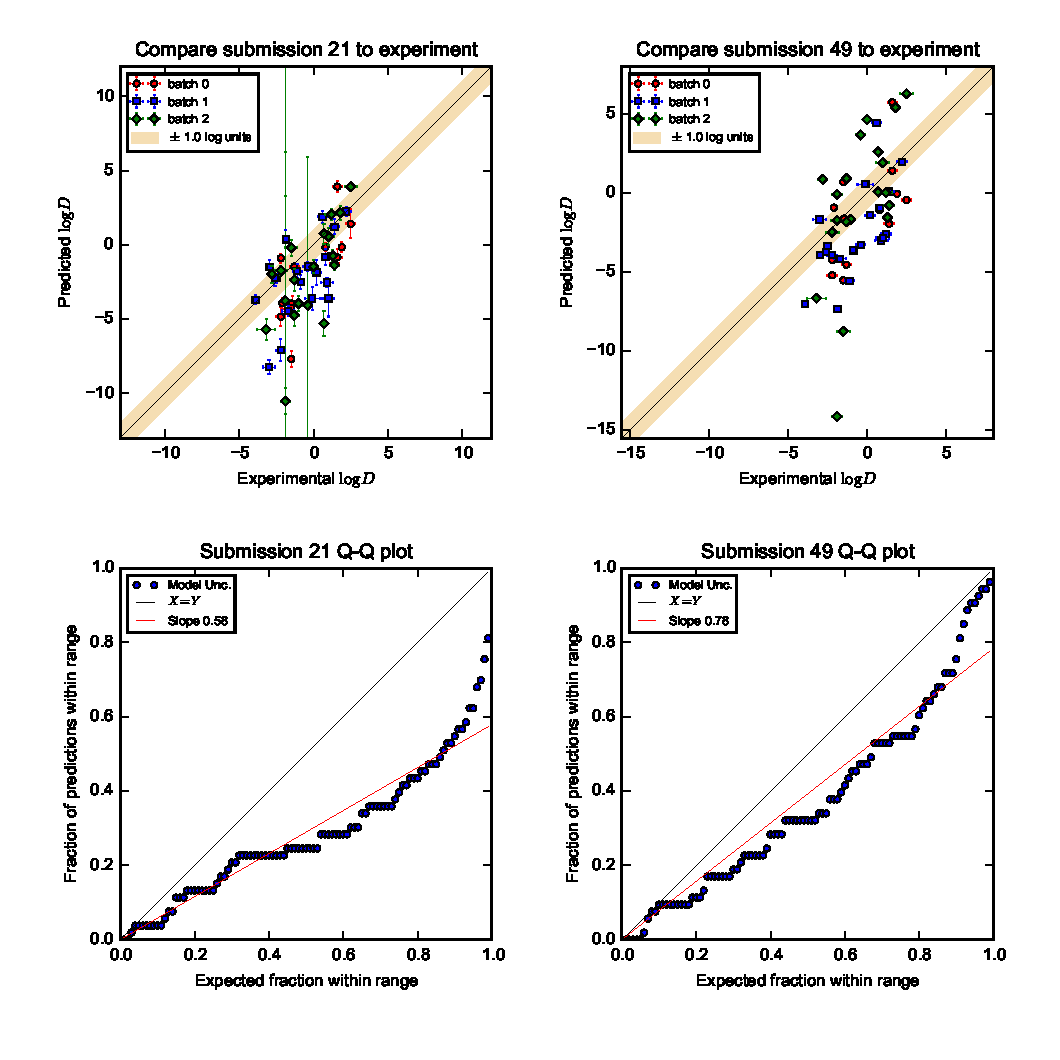
\includegraphics{ExamplePlots.eps}
\caption{These are examples of plots created for each set of predictions. They were chosen to try to represent the average submissions, those that were in the middle by most error metrics. a and b) comparison plots showing how predicted distribution coefficients compared to experiment for both groups. c,d) QQ Plots showing how their actual predictions were distributed compared to expectations given the model uncertainty.}
\label{examplePlots}       % I think they are all supposed to be named fig:#, but until we decide on an order i'm leaving my labels
\end{figure*}

% To compare each prediction set to experiment compare plots, QQ, error metric calculated for each prediction set
A total of six error metrics are used to evaluate all sets of predictions: root-mean-squared error (RMSE), average unsigned error (AUE), average signed error (ASE), Pearson's R (R), Kendall's tau (tau), and the slope from the QQ-plot (error slope) (Table \ref{groupStats}). 
For each group, we also created a plot comparing their predictions to experimental results.
A few example plots are provided (Fig. \ref{examplePlots}) these represent a typical submission, in that these groups were in the middle of the pack by most error metrics. 
Comparison and QQ-plots for every submission are available in the supporting information as well as error metric tables broken down by batch. 

% I think the histograms have to be two separate figures or take up an entire page, which seems a little unreasonable. 
% I'm fixing formatting on these, should have them in the next draft. 
% Histograms - RMS, AUE, ASE
\begin{figure*} % for 2 column use
% Insert figure
\caption{}
\label{histogramsAverage}       % I think they are all supposed to be named fig:#, but until we decide on an order i'm leaving my labels
\end{figure*}

% Histograms - R, tau, error slope
\begin{figure*} % for 2 column use
% Insert figure
\caption{}
\label{histogramsCorrelations}       % I think they are all supposed to be named fig:#, but until we decide on an order i'm leaving my labels
\end{figure*}

% histograms and batches
To help visualize all of the error metrics, the data was compiled into a histogram where results are sorted by what would be ideal for that metric (closest to 1 for error slope for example). 
These metrics are split into measurements of deviation from experiment (Fig. \ref{histogramsAverage}) and correlation with experiment (Fig. \ref{histogramsCorrelations}) distinctions which helped in identifying high performing groups. 
Most submissions included data for all three batches so these histograms are limited to those submissions. 
A total of eight submissions from two participants that only included data from batch 0, then an additional 5 submissions from 2 participants with only batches 0 and 1.
These submissions are indicated in Table \ref{groupStats} for clarity.
% More about how they would have done...
% Stefan Kast only submitted batch 0 results with EC-RISM type methods. 
% Julien Michel's group submitted 4 sets to just 0, 4 to 0 and 1, and 4 to 0, 1, and 2 with the same method labels, I did a quick check, I think they misunderstood the directions and submitted their data for batch 0, batch 0 and 1, and batch 0, 1, and 2, their numbers for the same method labels have identical results in the different submissions for the set of molecules I looked at. I haven't checked everything or asked Stefano, but I think that is what happened. 
% Gerhard Koenig had one set that they only did batch 0 and 1, but they have 7 other submissions so I think they're fine. 
%Kast's submissions were mostly middle (to upper middle) of the pack 

% Error Slope, only one participant (two submissions) did a good job with this % cite Andrew Paluch's paper if he is writing one
In considering the results for the error slope analysis, participants generally tend to do poorly estimating model uncertainty. 
The top three submissions are the only within uncertainty of 1, submissions 53 and 60 from Andrew Paluch % at location cite paper
and submission 43 from Gerhard Koenig % at location cite paper. 
% Double check their methods to see if they specifically comments on model uncertainty
Only one submission (40) significantly overestimated their model uncertainty. 
The rest are below 1, indicating a significant underestimation of the model uncertainty. 
% I will need to elaborate. ... 

% Kendall W if we decide to include it

\subsection{Prediction sets that performed most strongly}
\label{results:2}
\begin{figure*} % for 2 column use
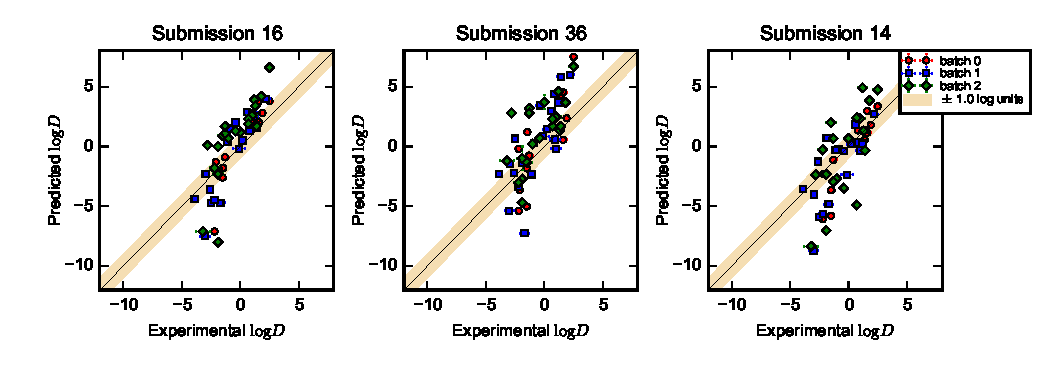
\includegraphics{BestGroups.eps}
\caption{}
\label{BestGroups}       % I think they are all supposed to be named fig:#, but until we decide on an order i'm leaving my labels
\end{figure*}
We want to consider how close to experiment RMSE/AUE and how well correlated with experiment tau/R

16 did best across both metric, COSMO-RS, brief statement about procedure

14 and 36 also did very well, making "top 10" by at least 3 of those 4 metrics, 14 is one of Frank Pickard's and 36 is Chris Fennell

but really null did best across the board so we have a lot of work to do... best RMSE over 2.0 log units and average around 3.5

\subsection{Null Hypothesis}
\label{results:3}
% I need to find a good citation, but I remember talking in Pharm 272 about how a "good" predictive method should do better than any null hypothesis. 
% good predictive method should be better than a "null" hypothesis. All molecules equally distribute between cyc and water so logD = 0.0
One way of evaluating predictive models is to compare them to a null hypothesis, or default result of some kind. 
In the case of distribution coefficients, we chose a null hypothesis where we assume all solute molecules distribute equally between cyclohexane and water, corresponding to a $\log D = 0$. 
We performed all error analyses discussed above on this pretend data set as a point of comparison. 


\subsection{Compounds that were difficult to accurately predict}

% Including the SMILES strings looks terrible in my opinion, maybe we could do 2d images if we have time or something
% Otherwise maybe I should just include 1 histogram plot of the AUE for the molecules and leave it at that. 
\label{results:4}
\begin{table}
\begin{tabular}{|c c c c c c c|}
\hline 
\multicolumn{7}{|c|}{{\small\textbf{Batch 0}}}\\ 
{\scriptsize 003: $ 1.7 \pm 0.2 $ } & {\scriptsize 015: $ 8.8 \pm 1.4 $ } & {\scriptsize 017: $ 3.0 \pm 0.3 $ } & {\scriptsize 020: $ 3.9 \pm 0.4 $ } & {\scriptsize 037: $ 7.5 \pm 1.3 $ } & {\scriptsize 045: $ 1.4 \pm 0.2 $ } & {\scriptsize 055: $ 2.7 \pm 0.2 $ } \\ 
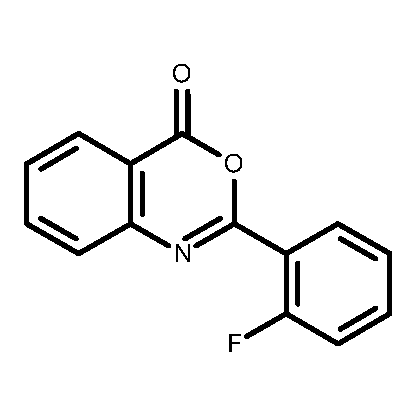
\includegraphics[width = 0.14\textwidth]{2DImages/SAMPL5_003.pdf} & 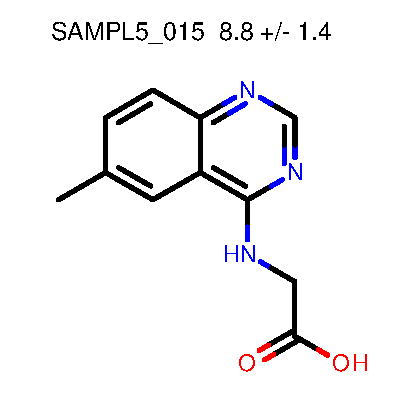
\includegraphics[width = 0.14\textwidth]{2DImages/SAMPL5_015.pdf} & 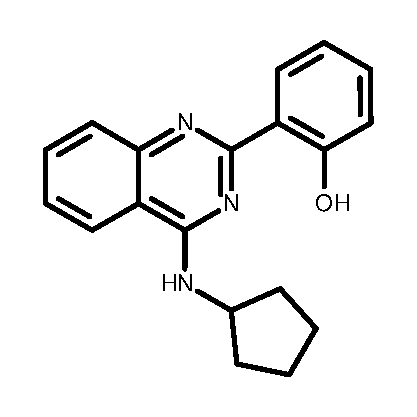
\includegraphics[width = 0.14\textwidth]{2DImages/SAMPL5_017.pdf} & 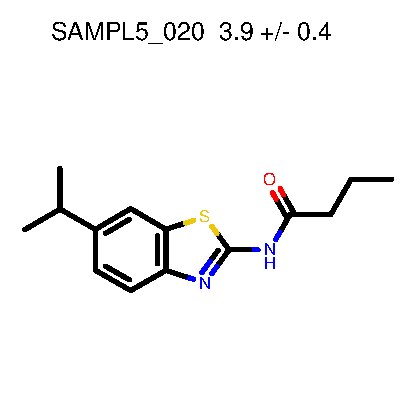
\includegraphics[width = 0.14\textwidth]{2DImages/SAMPL5_020.pdf} & 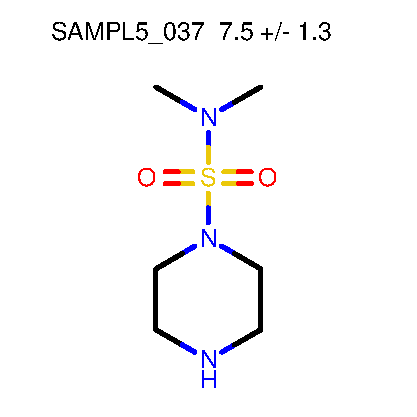
\includegraphics[width = 0.14\textwidth]{2DImages/SAMPL5_037.pdf} & 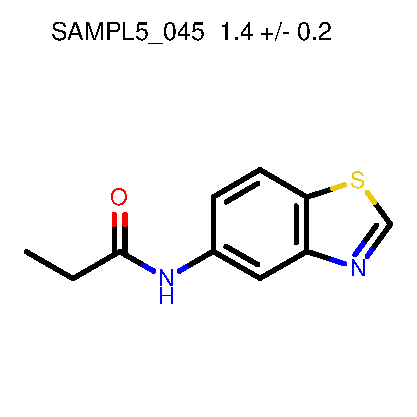
\includegraphics[width = 0.14\textwidth]{2DImages/SAMPL5_045.pdf} & 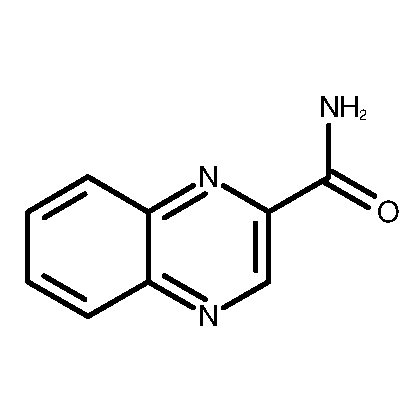
\includegraphics[width = 0.14\textwidth]{2DImages/SAMPL5_055.pdf} \\ 
{\scriptsize 058: $ 2.2 \pm 0.3 $ } & {\scriptsize 059: $ 1.8 \pm 0.2 $ } & {\scriptsize 061: $ 5.9 \pm 1.0 $ } & {\scriptsize 068: $ 2.7 \pm 0.3 $ } & {\scriptsize 070: $ 5.9 \pm 0.8 $ } & {\scriptsize 080: $ 2.6 \pm 0.2 $ } & \\ 
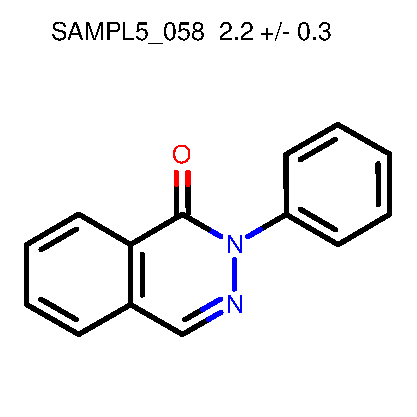
\includegraphics[width = 0.14\textwidth]{2DImages/SAMPL5_058.pdf} & 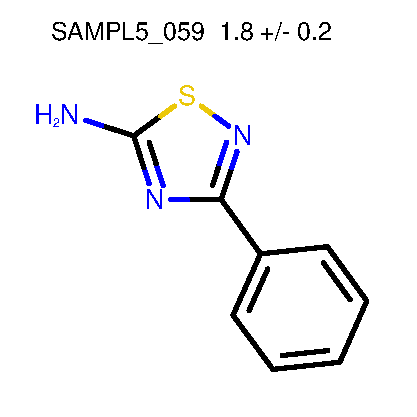
\includegraphics[width = 0.14\textwidth]{2DImages/SAMPL5_059.pdf} & 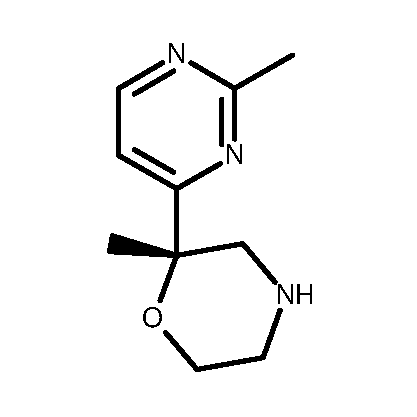
\includegraphics[width = 0.14\textwidth]{2DImages/SAMPL5_061.pdf} & 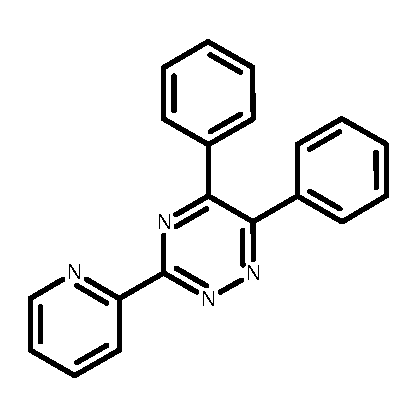
\includegraphics[width = 0.14\textwidth]{2DImages/SAMPL5_068.pdf} & 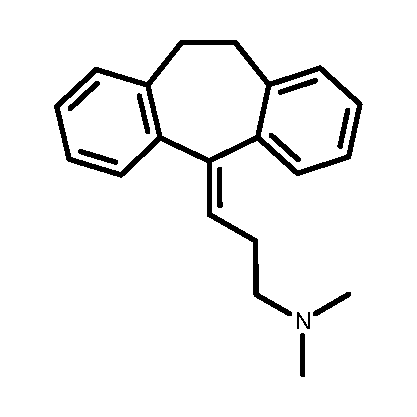
\includegraphics[width = 0.14\textwidth]{2DImages/SAMPL5_070.pdf} & 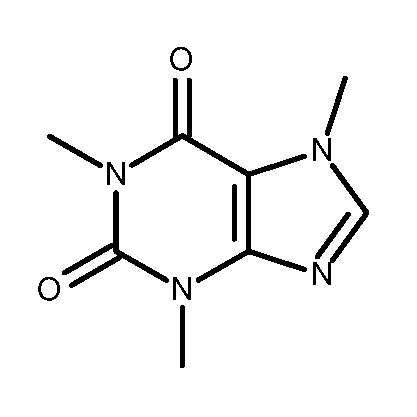
\includegraphics[width = 0.14\textwidth]{2DImages/SAMPL5_080.pdf} & \\ 
\hline 
\multicolumn{7}{|c|}{{\small\textbf{Batch 1}}}\\ 
{\scriptsize 004: $ 2.3 \pm 0.3 $ } & {\scriptsize 005: $ 2.6 \pm 0.3 $ } & {\scriptsize 007: $ 3.1 \pm 0.4 $ } & {\scriptsize 010: $ 7.8 \pm 1.6 $ } & {\scriptsize 011: $ 7.1 \pm 1.3 $ } & {\scriptsize 021: $ 2.2 \pm 0.2 $ } & {\scriptsize 026: $ 8.0 \pm 1.7 $ } \\ 
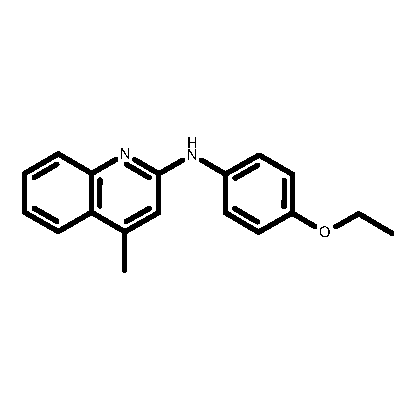
\includegraphics[width = 0.14\textwidth]{2DImages/SAMPL5_004.pdf} & 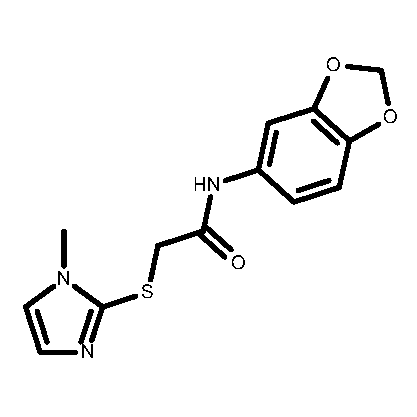
\includegraphics[width = 0.14\textwidth]{2DImages/SAMPL5_005.pdf} & 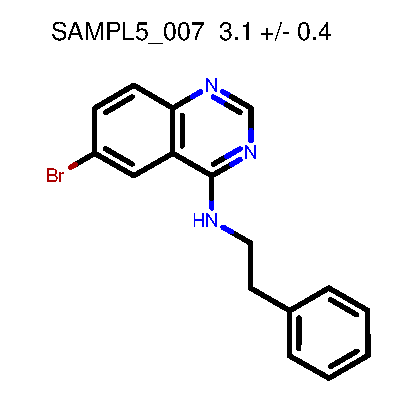
\includegraphics[width = 0.14\textwidth]{2DImages/SAMPL5_007.pdf} & 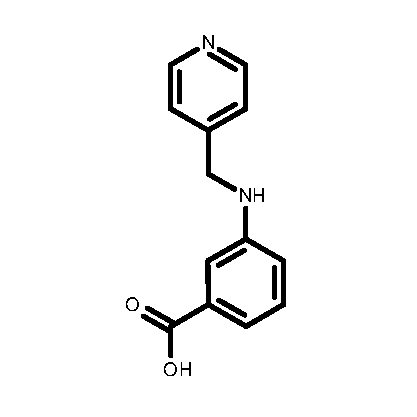
\includegraphics[width = 0.14\textwidth]{2DImages/SAMPL5_010.pdf} & 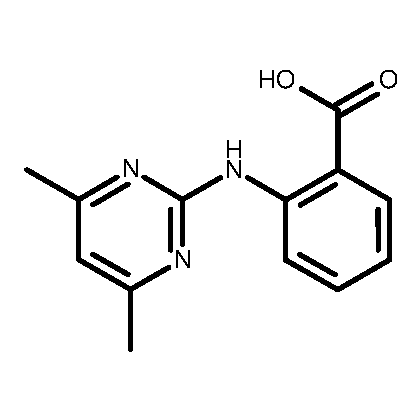
\includegraphics[width = 0.14\textwidth]{2DImages/SAMPL5_011.pdf} & 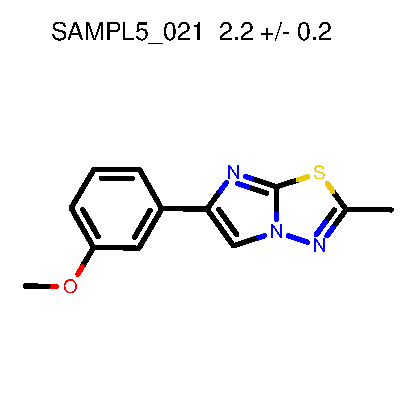
\includegraphics[width = 0.14\textwidth]{2DImages/SAMPL5_021.pdf} & 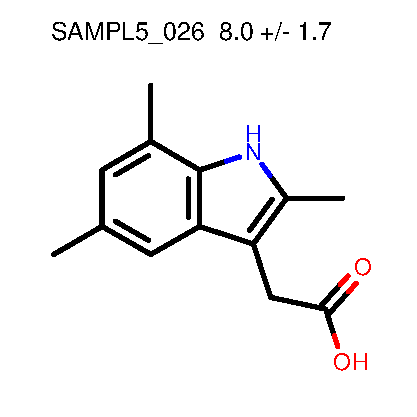
\includegraphics[width = 0.14\textwidth]{2DImages/SAMPL5_026.pdf} \\ 
{\scriptsize 027: $ 3.4 \pm 0.3 $ } & {\scriptsize 042: $ 3.2 \pm 0.4 $ } & {\scriptsize 044: $ 3.7 \pm 0.4 $ } & {\scriptsize 046: $ 2.7 \pm 0.4 $ } & {\scriptsize 047: $ 2.1 \pm 0.3 $ } & {\scriptsize 048: $ 2.7 \pm 0.3 $ } & {\scriptsize 056: $ 3.5 \pm 0.3 $ } \\ 
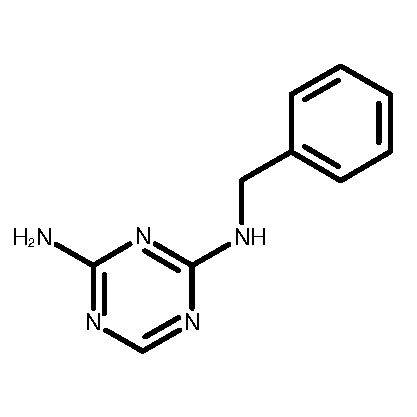
\includegraphics[width = 0.14\textwidth]{2DImages/SAMPL5_027.pdf} & 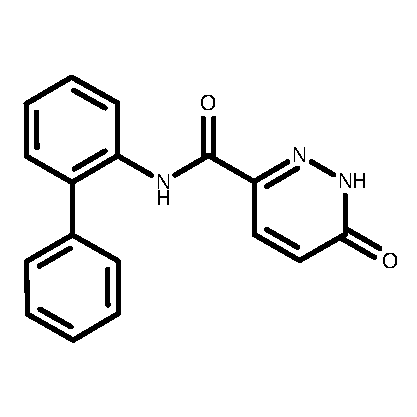
\includegraphics[width = 0.14\textwidth]{2DImages/SAMPL5_042.pdf} & 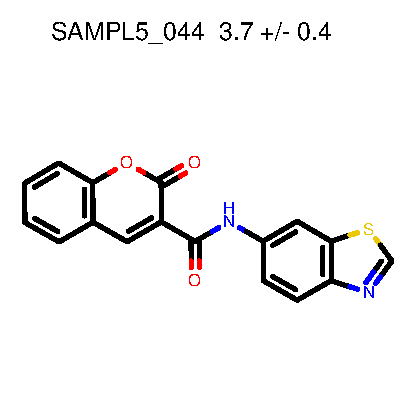
\includegraphics[width = 0.14\textwidth]{2DImages/SAMPL5_044.pdf} & 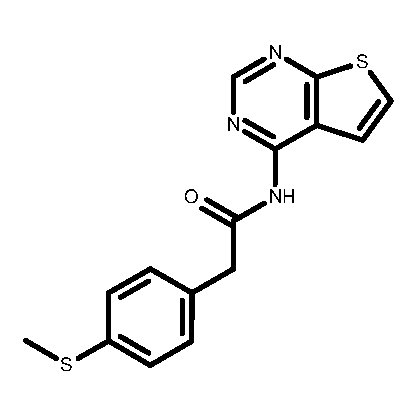
\includegraphics[width = 0.14\textwidth]{2DImages/SAMPL5_046.pdf} & 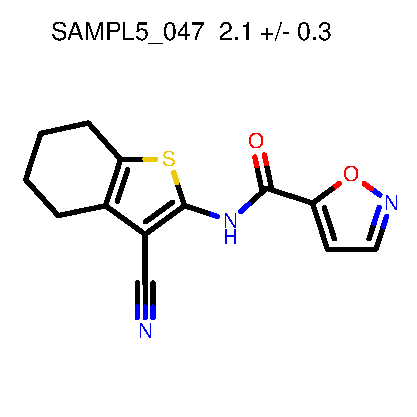
\includegraphics[width = 0.14\textwidth]{2DImages/SAMPL5_047.pdf} & 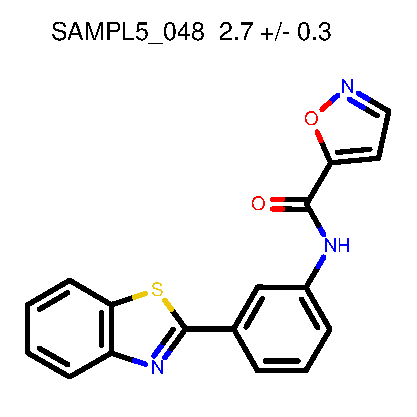
\includegraphics[width = 0.14\textwidth]{2DImages/SAMPL5_048.pdf} & 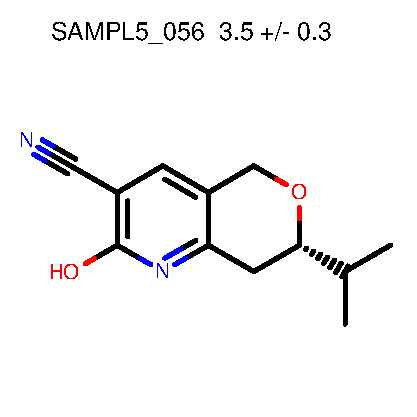
\includegraphics[width = 0.14\textwidth]{2DImages/SAMPL5_056.pdf} \\ 
{\scriptsize 060: $ 6.7 \pm 1.6 $ } & {\scriptsize 063: $ 6.7 \pm 1.0 $ } & {\scriptsize 071: $ 2.8 \pm 0.3 $ } & {\scriptsize 072: $ 4.9 \pm 0.7 $ } & {\scriptsize 081: $ 6.0 \pm 0.8 $ } & {\scriptsize 090: $ 2.8 \pm 0.3 $ } & \\ 
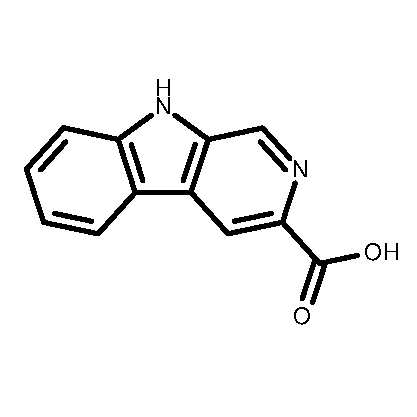
\includegraphics[width = 0.14\textwidth]{2DImages/SAMPL5_060.pdf} & 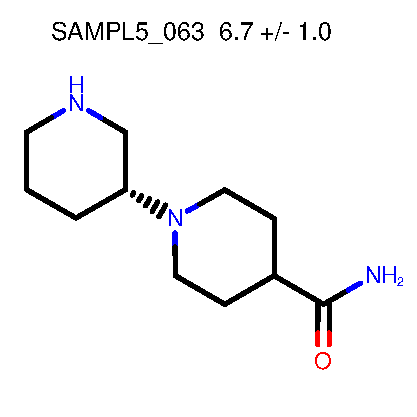
\includegraphics[width = 0.14\textwidth]{2DImages/SAMPL5_063.pdf} & 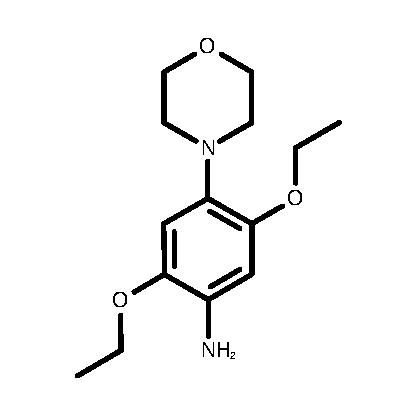
\includegraphics[width = 0.14\textwidth]{2DImages/SAMPL5_071.pdf} & 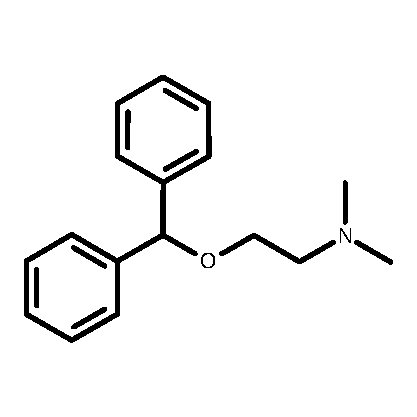
\includegraphics[width = 0.14\textwidth]{2DImages/SAMPL5_072.pdf} & 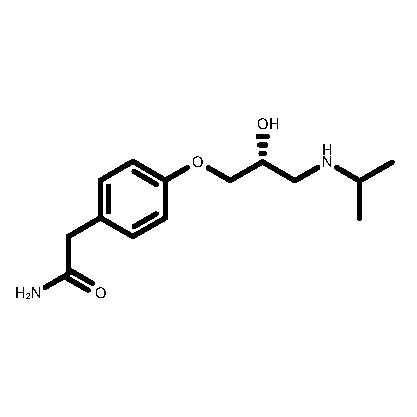
\includegraphics[width = 0.14\textwidth]{2DImages/SAMPL5_081.pdf} & 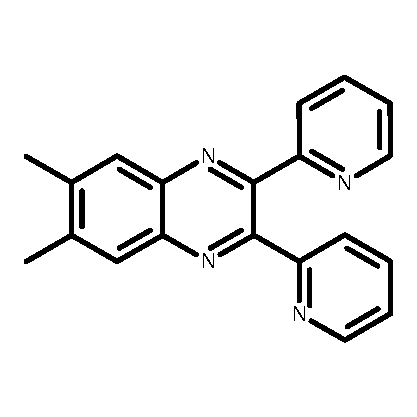
\includegraphics[width = 0.14\textwidth]{2DImages/SAMPL5_090.pdf} & \\ 
\hline 
\multicolumn{7}{|c|}{{\small\textbf{Batch 2}}}\\ 
{\scriptsize 002: $ 2.5 \pm 0.2 $ } & {\scriptsize 006: $ 2.7 \pm 0.4 $ } & {\scriptsize 013: $ 3.1 \pm 0.3 $ } & {\scriptsize 019: $ 3.1 \pm 0.4 $ } & {\scriptsize 024: $ 3.0 \pm 0.4 $ } & {\scriptsize 033: $ 3.0 \pm 0.3 $ } & {\scriptsize 049: $ 2.1 \pm 0.2 $ } \\ 
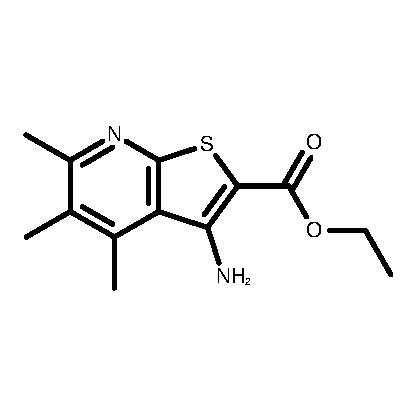
\includegraphics[width = 0.14\textwidth]{2DImages/SAMPL5_002.pdf} & 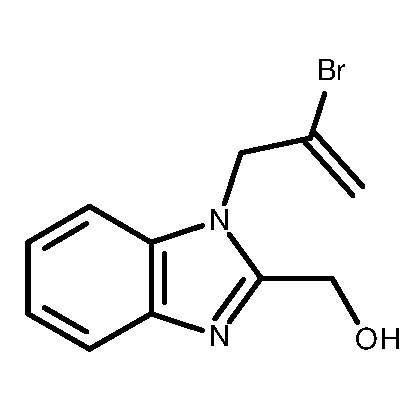
\includegraphics[width = 0.14\textwidth]{2DImages/SAMPL5_006.pdf} & 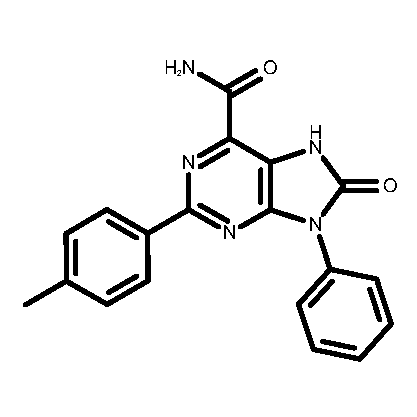
\includegraphics[width = 0.14\textwidth]{2DImages/SAMPL5_013.pdf} & 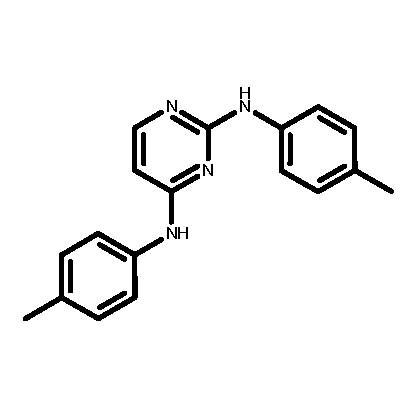
\includegraphics[width = 0.14\textwidth]{2DImages/SAMPL5_019.pdf} & 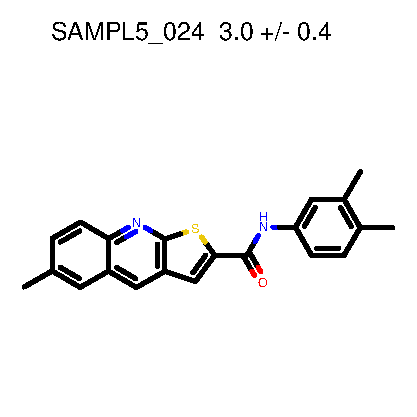
\includegraphics[width = 0.14\textwidth]{2DImages/SAMPL5_024.pdf} & 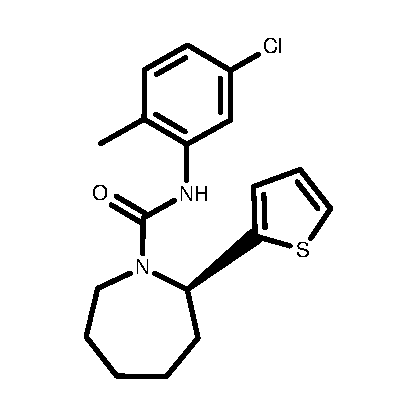
\includegraphics[width = 0.14\textwidth]{2DImages/SAMPL5_033.pdf} & 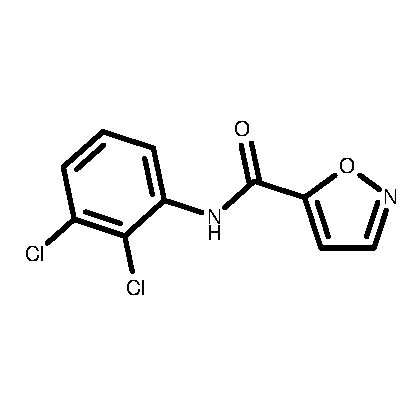
\includegraphics[width = 0.14\textwidth]{2DImages/SAMPL5_049.pdf} \\ 
{\scriptsize 050: $ 5.6 \pm 0.4 $ } & {\scriptsize 065: $ 5.3 \pm 0.5 $ } & {\scriptsize 067: $ 4.5 \pm 0.6 $ } & {\scriptsize 069: $ 3.9 \pm 0.5 $ } & {\scriptsize 074: $ 6.6 \pm 0.4 $ } & {\scriptsize 075: $ 4.8 \pm 0.6 $ } & {\scriptsize 082: $ 5.1 \pm 0.6 $ } \\ 
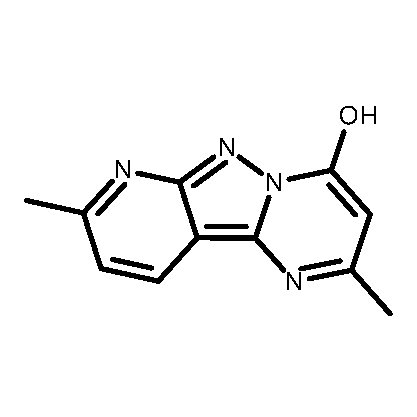
\includegraphics[width = 0.14\textwidth]{2DImages/SAMPL5_050.pdf} & 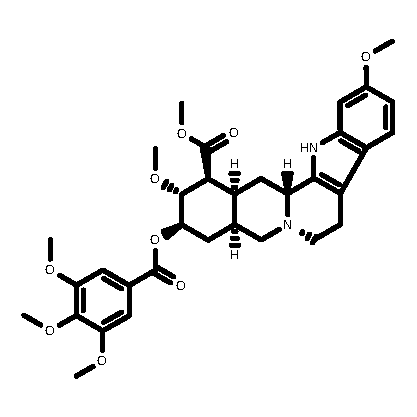
\includegraphics[width = 0.14\textwidth]{2DImages/SAMPL5_065.pdf} & 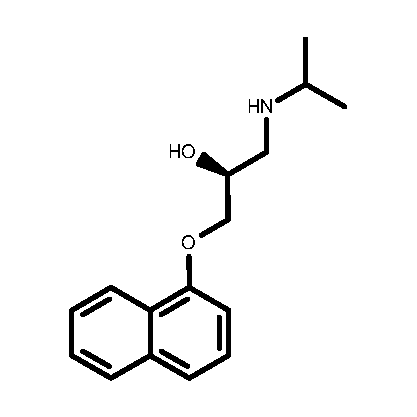
\includegraphics[width = 0.14\textwidth]{2DImages/SAMPL5_067.pdf} & 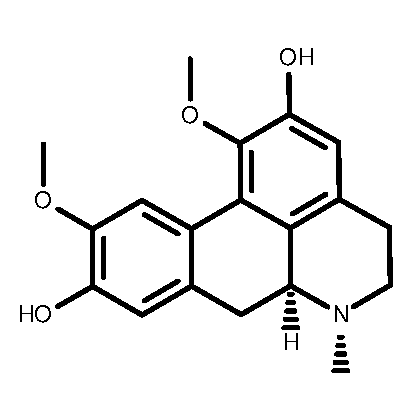
\includegraphics[width = 0.14\textwidth]{2DImages/SAMPL5_069.pdf} & 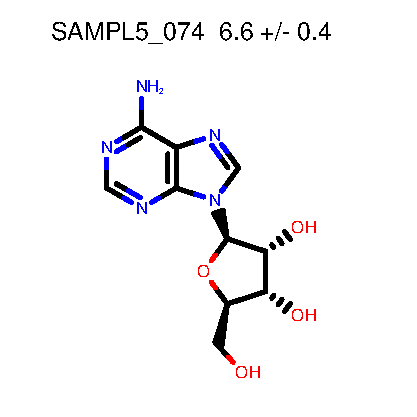
\includegraphics[width = 0.14\textwidth]{2DImages/SAMPL5_074.pdf} & 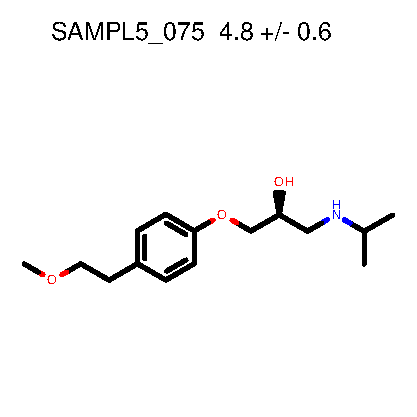
\includegraphics[width = 0.14\textwidth]{2DImages/SAMPL5_075.pdf} & 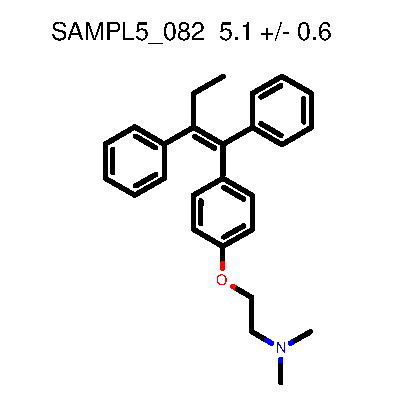
\includegraphics[width = 0.14\textwidth]{2DImages/SAMPL5_082.pdf} \\ 
{\scriptsize 083: $ 8.4 \pm 0.7 $ } & {\scriptsize 084: $ 3.6 \pm 0.5 $ } & {\scriptsize 085: $ 2.8 \pm 0.3 $ } & {\scriptsize 086: $ 4.5 \pm 0.6 $ } & {\scriptsize 088: $ 2.9 \pm 0.4 $ } & {\scriptsize 092: $ 3.9 \pm 0.4 $ } & \\ 
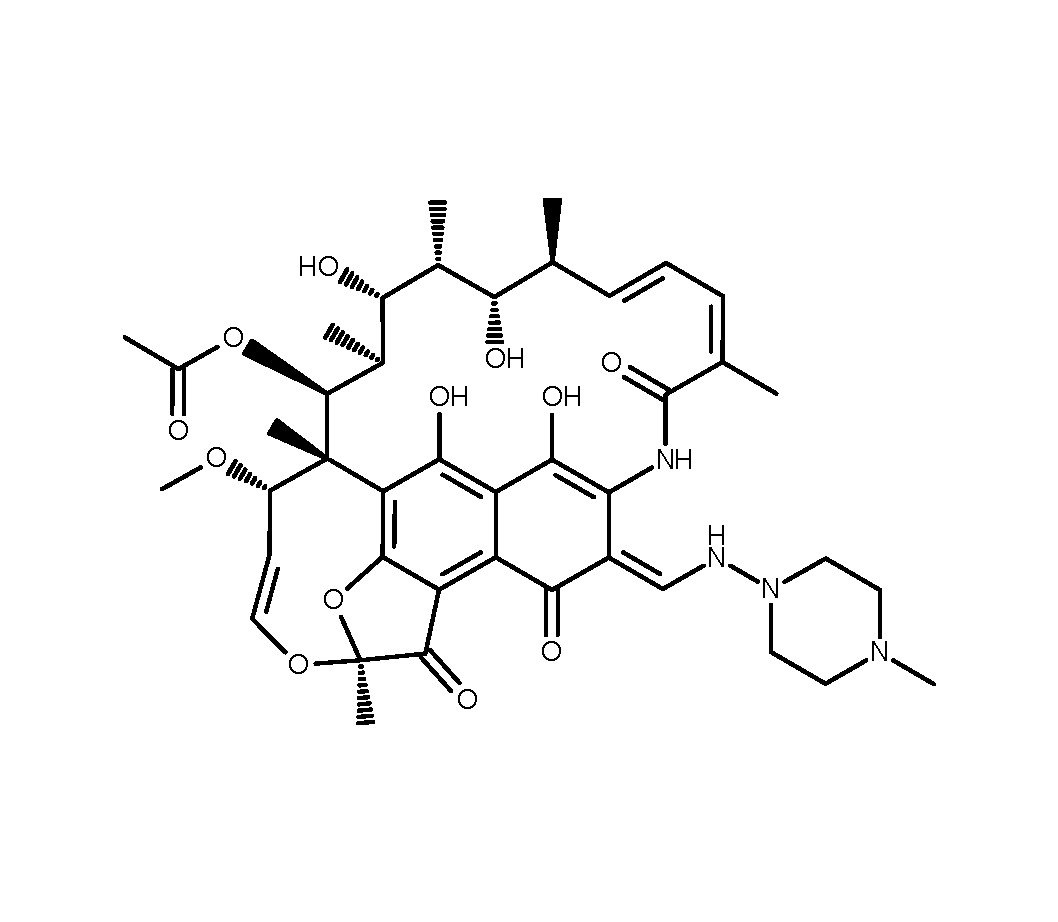
\includegraphics[width = 0.14\textwidth]{2DImages/SAMPL5_083.pdf} & \includegraphics[width = 0.14\textwidth]{2DImages/SAMPL5_084.pdf} & \includegraphics[width = 0.14\textwidth]{2DImages/SAMPL5_085.pdf} & \includegraphics[width = 0.14\textwidth]{2DImages/SAMPL5_086.pdf} & \includegraphics[width = 0.14\textwidth]{2DImages/SAMPL5_088.pdf} & \includegraphics[width = 0.14\textwidth]{2DImages/SAMPL5_092.pdf} & \\ 
\hline
\end{tabular}

\label{MoleculeTable}
\caption{A complete list of compounds used in the SAMPL5, sorted by batch. The mean unsigned error, reported in log units, was calculated with all predictions for that compound.} 
\end{table}

Full error analysis repeated for individual molecules, there aren't very many "simple" molecules, almost all have hetro atoms and rotatable bonds...

about 5-10 worst, I'm looking into if there are trends in number of tautomer or functional group similarities...

about 5-10 best, still looking for trends, we know 083, 074. 015 also did poorly amino acid? I don't know why that would cause more problems in general. 

% possibly a paragraph about MW, # of rotatable bonds, or # of tautomers (no tautomer trend yet...)

\subsection{Classes of methods...}
\label{results:5}
Broad range of methods, split into classes: MD all atom, MD hybrid, quantum?, Anything similar to COSMO? % I'm still reading and trying to understand methods
Pie chart by number maybe?

Clear trends on which are doing well? 

\subsection{Mobley group prediction results}
\label{results:6}

% Our comparison plots
\begin{figure*}
% insert figure 
\caption{Plots showing our predictions compared to experiment. a) submission 39 to SAMPL5, with no tautomer correction. b) distribution coefficient corrected from calculated partition coefficient based on pKas. c) distribution coefficient correct from calculated partition coefficient with state penalties }
\label{myComparisons}       % Give a unique label
\end{figure*}

% How did logP do, not bad in general, include our plots
We submitted a set of blind predictions (39) to the challenge. 
Solvation free energies were calculated using GROMACS with GAFF and AM1-BCC charges. 
The initial set of predictions were partition coefficients, determined from the difference in solvation free energies without correcting for variation in tautomers. 
39 was within the top 15 %(check this) 
submissions for all error metrics.  
% Double check numbers, slight bias for cyclohexane to water from average signed error

After the challenge we explored how correcting for protonation states would have affected the our initial predictions. 
The first set of corrections involved calculating the pKa for each molecule using Schrodinger's Epik tool. 
Next, $\log D$ was calculated using the pKa and partition coefficient determined in submission 39 using eqn. % get reference
For compounds with more than one pKa, the one which caused the largest change in $\log D$ was used, this would represent the most acidic proton leaving or most basic functional group becoming protonated. % this is a confusing sentence
This correction showed a slight improvement by most error metrics (Table % ref table) 
including a decrease in the average error (value) indicating less bias toward concentration. 

For the next set of corrections, we used Schrodinger's Ligprep tool to calculate a state penalty, which gives the relative population of tautomers in water at a given pH. % ick
The state penalty was used to correct the concentration in the aqueous layer, according to eqn. % reference if I have one
State penalties improved predictions from the original partition coefficient coefficients and showed a slight improvement over the pKa corrections (Fig. \ref{myComparisons}). 
% Expand here...
Both of these correction methods only adjust the concentration in the aqueous layer, however there may be tautomer affects that also affect the concentration in cyclohexane as well. 
There are a few molecules where the state penalty correction caused a significant bias for the concentration in the aqueous layer (SAMPL5\_050). % I need to double check the others
One explanation for these extreme examples is that the solute might have other neutral tautomers that would affect the concentration in cyclohexane, which we did not correct for. 
% add a sentence or two here to conclude this


\subsection{Reanalysis of difficult tautomers} % I don't like difficult here
\label{results:7}
% It was clear from epik and discussions with other SAMPL5 participants (cite Klamt?)  that 050 and 083 had dominant tautomers other than provided SMILE
From our tautomer enumeration and discussions with other SAMPL5 participants % cite Andreas and maybe Frank, look at e-mail
it became clear that the provided SMILES string may not be the most popular %???
tautomeric form of the molecule. 
If we could perfectly calculate solvation free energies and tautomer populations in both solvents, starting tautomer should not effect the final calculated distribution coefficient.  
Our initial solvation free energy calculations used provided SMILES strings without any consideration of other tautomers.
To explore how this may have affected our $\log D$ calculation, we decided to repeat a few solvation free energy calculations with different tautomers. 
We repeated calculations with different tautomers of SAMPL5\_050 and SAMPL5\_083 that could be present in both the water and cyclohexane solutions. 
To explore how the tautomer used to calculate the solvation free energy might effect the estimate of a distribution coefficient. 

% I got slightly distracted playing with table formatting, I'm working on coding it out and copy and paste it here. 
\begin{table}
\begin{tabular}{l | l l | l l}
\hline
& \multicolumn{2}{|c|}{SAMPL5\_050} & \multicolumn{2}{c}{SAMPL5\_083} \\
& tautomer 1 & tautomer 2 & tautomer 1 & tautomer 2 \\
\hline
$\Delta G_{hydration}$ & $ 1 \pm 1 $ &  $ 1 \pm 1$ &  $1 \pm 1$ &  $1 \pm 1$ \\
$\Delta G_{cyclohexane}$ & $ 1 \pm 1 $ &  $ 1 \pm 1$ &  $1 \pm 1$ &  $1 \pm 1$ \\
$\log P_{cyc/wat}$ & $ 1 \pm 1 $ &  $ 1 \pm 1$ &  $1 \pm 1$ &  $1 \pm 1$ \\
Correction & $ 1 \pm 1 $ &  $ 1 \pm 1$ &  $1 \pm 1$ &  $1 \pm 1$ \\
$\log D_{cyc/water}$ & $ 1 \pm 1 $ &  $ 1 \pm 1$ &  $1 \pm 1$ &  $1 \pm 1$ \\
\hline
experimental $\log D$ & \multicolumn{2}{|c|}{$1 \pm 1$} & \multicolumn{2}{c}{$1 \pm 1$} \\
\hline
\end{tabular}
\label{tautomerChanges}
\caption{Simulations with different tautomers...}
\end{table}
% Possibly 2d images of the two tautomers...


We reran these tautomers to calculate solvation free energies, used state penalty %results in a table probably (or maybe a figure like the one I made for erythromycin in the logP paper)

Generally hard to tell if its tautomer enumeration that isn't good or the solvation free energies

\subsection{Considering how solvent interactions could possibly affect results} % I don't like difficult here
\label{results:7}

\section{Conclustion}
\label{conclusions}

Overall, range of methods and performance

Compare to dGhydration in past SAMPL challenges? using average errors, possibly what methods/FF are top ranked?

Tautomer and/or pKa predictions are going to be an important part of improving these

We, as a communitee, need to improve error estimation, both how we do and how we evaluate it...

logP/logD seem to be good options for future blind challenges

\begin{acknowledgements} % this is just a list so we don't forget anyone
John Chodera and Bas MSKCC
Andreas Klamt
Chris Fennell
Samuel Genheden
D3R team
people who set up the automated submission system %they are gods in my opion =]


\end{acknowledgements}

\subsection{Available in supporting info} % This is a list for myself, it will all be archived or provided with a link to to somewhere on the web
things provided to participants
all scripts used for error analysis
all participant files? Can we include the anonymous one? 
triple check no names/e-mails/institutions/etc in the final submitted data
all plots not in the paper
all input/output files for schrodinger calculations
all input files and results files for 'logP' calculations, tautomer redos, box size simulations (PME too?) 
example MDP and run scripts
 


% BibTeX users please use one of
%\bibliographystyle{spbasic}      % basic style, author-year citations
%\bibliographystyle{spmpsci}      % mathematics and physical sciences
%\bibliographystyle{spphys}       % APS-like style for physics
%\bibliography{}   % name your BibTeX data base

%\subsection{Subsection title}
%\label{sec:2}
% Examples from the JCAMD template 
% Text with citations \cite{RefB} and \cite{RefJ}.
% (see Sect.~\ref{sec:1}).
% \paragraph{Paragraph headings} Use paragraph headings as needed.

% For one-column wide figures use
%\begin{figure}
% Use the relevant command to insert your figure file.
% For example, with the graphicx package use
%  \includegraphics{example.eps}
% figure caption is below the figure
%\caption{Please write your figure caption here}
%\label{fig:1}       % Give a unique label
%\end{figure}
%
% For two-column wide figures use
%\begin{figure*}
% Use the relevant command to insert your figure file.
% For example, with the graphicx package use
%  \includegraphics[width=0.75\textwidth]{example.eps}
% figure caption is below the figure
%\caption{Please write your figure caption here}
%\label{fig:2}       % Give a unique label
%\end{figure*}
%
% For tables use
%\begin{table}
% table caption is above the table
%\caption{Please write your table caption here}
%\label{tab:1}       % Give a unique label
% For LaTeX tables use
%\begin{tabular}{lll}
%\hline\noalign{\smallskip}
%first & second & third  \\
%\noalign{\smallskip}\hline\noalign{\smallskip}
%number & number & number \\
%number & number & number \\
%\noalign{\smallskip}\hline
%\end{tabular}
%\end{table}


\end{document}

